\documentclass[onecolumn,a4paper,10pt]{report}
%\documentclass[12pt,a4paper,twoside]{book} %twoside distingue página par de ímpar
\usepackage[utf8]{inputenc}
\usepackage[portuges]{babel} %para separar sílabas em Português, etc...
\usepackage[usenames,dvipsnames]{color} % para letras e caixas coloridas
\usepackage{latexsym} %para fazer $\Box$ no \LaTeX2$\epsilon$
\usepackage{makeidx} % índice remissivo
\usepackage{amstext} %texto em equações: $... \text{} ...$
\usepackage{float}
\usepackage{theorem}
\usepackage{tabularx} %tabelas ocupando toda a página
\usepackage[all]{xy}
\usepackage{a4wide} %correta formatação da página em A4
\usepackage{indentfirst} %adiciona espaços no primeiro parágrafo

\usepackage{graphics,amssymb,amsfonts,amsmath}
\usepackage{tikz}
\usepackage{enumerate,hyperref}
\usepackage{palatino}
\usepackage{ragged2e}
\usepackage{minted}
\usepackage{booktabs}
\usepackage{verbatim}
\usepackage[export]{adjustbox}
\usepackage{tikz}                   
\usepackage{xcolor}
\usepackage{textcomp} % para usar \textdegree
\usepackage{setspace}
\usetikzlibrary{shadows}

\newminted{java}{bgcolor=cyan!10}

\definecolor{cinza}{gray}{.8}
\definecolor{branco}{gray}{1}
\definecolor{preto}{gray}{0}
\definecolor{verdemusgo}{rgb}{.3,.7,.5}
\definecolor{vinho}{cmyk}{0,1,1,.5}
%\setcounter{secnumdepth}{1}
%\renewcommand{\thesection}{\textcolor{preto}{\arabic{section}}}
%\renewcommand{\thepage}{\textcolor{preto}{\color{preto}{{\scriptsize}}}}
{\theorembodyfont{\upshape}
\newtheorem{Dem}{Demonstração}[chapter]}
\newtheorem{Ex}{Exemplo}[chapter]
\newtheorem{Exer}{Exercício}
\newtheorem{Lista}{Lista de exercícios}
\newtheorem{Def}{Definição}[chapter]

\newtheorem{Pro}{Proposição}[chapter]
\newtheorem{Ax}{Axioma}[chapter]
\newtheorem{Teo}{Teorema}[chapter]
\newtheorem{Cor}{Corolário}[chapter]
\newtheorem{Cas}{Caso}[subsection]
\newtheorem{lema}{Lema}[chapter]
\newtheorem{que}{Questão}[chapter]
\newcommand{\dem}{\noindent{\bf Demonstração:}}
\newcommand{\sol}{\noindent{\it Solução.}}
\newcommand{\nota}{\noindent{\bf Notação:}}
\newcommand{\ex}{\noindent{\bf Exemplos}}
\newcommand{\Obs}{\noindent{\bf Observação:}}
\newcommand{\fim}{\hfill $\blacksquare$}
\newcommand{\ig}{\,\, = \,\,}
\newcommand{\+}{\, + \,}
\newcommand{\m}{\, - \,}
\newcommand{\I}{\mbox{$I\kern-0.40emI$}}
\newcommand{\Z}{\mbox{Z$\kern-0.40em$Z}}
\newcommand{\Q}{\mbox{I$\kern-0.60em$Q}}
\newcommand{\C}{\mbox{I$\kern-0.60em$C}}
\newcommand{\N}{\mbox{I$\kern-0.40em$N}}
\newcommand{\R}{\mbox{I$\kern-0.40em$R}}
\newcommand{\Ro}{\rm{I\!R\!}}
\newcommand{\disp}{\displaystyle}
\newcommand{\<}{\hspace*{-0.4cm}}
\newcommand{\ds}{\displaystyle}
\newcommand{\ov}{\overline}
\newcommand{\aj}{\vspace*{-0.2cm}}
\newcommand{\pt}{\hspace{-1mm}\times\hspace{-1mm}}
\newcommand{\cm}{\mbox{cm}}
\newcommand{\np}{\mbox{$\in \kern-0.80em/$}}
\newcommand{\tg} {\mbox{tg\,}}
\newcommand{\ptm}{\hspace{-0.4mm}\cdot\hspace{-0.4mm}}
\newcommand{\arc}{\stackrel{\;\;\frown}}
\newcommand{\rad}{\;\mbox{rad}}
\newcommand{\esp}{\;\;\;\;}
\newcommand{\sen}{\mbox{sen\,}}
\newcommand{\grau}{^{\mbox{{\scriptsize o}}}}
\newcommand{\real} {\mbox{$I\kern-0.60emR$}}
\newcommand{\vetor}{\stackrel{\color{vinho}\vector(1,0){15}}}
\newcommand{\arctg}{\mbox{arctg\,}}
\newcommand{\arcsen}{\mbox{arcsen\,}}
\newcommand{\ordinal}{^{\underline{\scriptsize\mbox{\rmo}}}}
\newcommand{\segundo}{$2^{\underline{o}}$ }
\newcommand{\primeiro}{$1^{\underline{o}}$ }
\newcommand{\nee}{\mbox{$\;=\kern-0.90em/\;$}}

\setlength{\parskip}{0.0cm} %espaco entre parágrafos
\setlength{\oddsidemargin}{-1cm} %margem esquerda das páginas
%\setlength{\unitlength}{3cm} %tamanho da figura criada
\linespread{1.5} %distância entre linhas
\setlength{\textheight}{25cm} %distância entre a primeira e última linha do texto(comprimento do texto)
\setlength{\textwidth}{18cm} %indica a largura do texto
\topmargin=-2cm %margem superior entre topo da página e o cabeçalho
%\headsep=0.5cm %distãncia entre o cabeçalho e o corpo do texto
%\setlength{\footskip}{27pt} %distãncia da última linha ao número da página
%\evensidemargin=-0.2in %margem esquerda das páginas pares
%\marginparwidth=1.7in %tamanho das notas de margem
%\marginparsep=0.2in %distância entre a margem direita e as notas de margem
%\topmargin=0cm
%\stackrel{\frown}{AB}

\begin{document}
\singlespacing

\begin{center}
Pontifícia Universidade Católica do Rio Grande do Sul (PUCRS)\\
Escola Politécnica\\
Disciplina: Fundamentos de Programação - Professor: Roland Teodorowitsch\\
26 de outubro de 2022
\end{center}

\begin{center}
\textbf{Lista de Exercícios - Unidade 5: Métodos}
\end{center}

\begin{enumerate}

\item Escreva um método em Java que recebe dois parâmetros inteiros \texttt{a} e \texttt{b} e calcula o valor de \texttt{a} elevado na potência \texttt{b}, retornando um valor inteiro e usando somas sucessivas, sem usar \texttt{Math.pow}.\\
{\tiny Autor: Roland Teodorowitsch}

\item Escreva métodos em Java para cada uma das seguintes descrições:
\begin{enumerate}[a.]
	\item Calcular o maior valor de dois valores inteiros.
	\item Computar o menor valor de três valores reais.
	\item Verificar se um número inteiro é um número primo, retornando \texttt{true} se for ou \texttt{false} em caso contrário.
	\item Receber duas cadeias de caracteres (\texttt{String}) e verificar se a segunda está contida dentro da primeira.
	\item Receber duas cadeias de caracteres (\texttt{String}) e verificar quantas vezes a segunda cadeia de caracteres está contida dentro da primeira. % Roland
	\item Receber uma cadeia de caracteres (\texttt{String}) e retornar esta cadeia de forma invertida.
	\item Receber uma cadeia de caracteres (\texttt{String}) e verificar se esta cadeia de caracteres é um palíndromo, retornando \texttt{true} se for, ou \texttt{false} em caso contrário.
	\item Calcular o saldo total de uma conta com determinado valor inicial, determinada taxa de juros anual e determinado número de anos de aplicação.
	\item Determinar o número de dias de determinado ano. % Roland
	\item Determinar o número de dias de determinado mês. % Roland
	\item Determinar o dia da semana de determinado dia, mês e ano (como uma cadeia de caracteres como ``segunda-feira'').
	\item Gerar um valor inteiro entre 1 e n.
\end{enumerate}
{\tiny Adaptado de: Horstmann (2013, p. 235)}

\item Analise as seguintes afirmações e verifique se elas são Verdadeiras ou Falsas:
\begin{enumerate}[a.]
	\item Um método tem sempre exatamente um valor de retorno.
	\item Um método deve ter pelo menos um valor de retorno.
	\item Um método pode ter no máximo um valor de retorno.
	\item Um método com valor de retorno \texttt{void} nunca tem um comando \texttt{return}.
	\item Quando o comando \texttt{return} é executado, a execução do método é concluída imediatamente.
	\item Um método com valor de retorno \texttt{void} deve imprimir um resultado.
	\item Um método sem variáveis paramétricas sempre retorna o mesmo valor.
\end{enumerate}
{\tiny Adaptado de: Horstmann (2013, p. 235-236)}

\newpage
\item Considere os seguintes métodos:
\begin{javacode}
public static double f(double x) { return g(x) + Math.sqrt(h(x)); }
public static double g(double x) { return 4 * h(x); }
public static double h(double x) { return x * x + k(x) - 1; }
public static double k(double x) { return 2 * (x + 1); }
\end{javacode}
Sem compilar ou executar este código em um programa, determine os resultados das seguintes chamadas de métodos:
\begin{enumerate}[a.]
	\item \texttt{double x1 = f(2);}
	\item \texttt{double x2 = g(h(2));}
	\item \texttt{double x3 = k(g(2) + h(2));}
	\item \texttt{double x4 = f(0) + f(1) + f(2);}
	\item \texttt{double x5 = f(-1) + g(-1) + h(-1) + k(-1);}
\end{enumerate}
{\tiny Adaptado de: Horstmann (2013, p. 236)}

\item Escreva um método em Java para converter um número de telefone que possua letras (tal como ``1-800-FLOWERS'') em um número de telefone real, com os respectivos números nos lugares das letras. Use as letras padrão em um teclado de telefone.
\begin{figure}[H]
	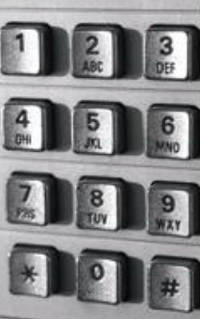
\includegraphics[height=3cm,center]{pucrs-ep-fprog-unidade_05-metodos-lista_de_exercicios-teclado.jpg}
\end{figure}
{\tiny Adaptado de: Horstmann (2013, p. 236)}

\item Para cada variável no programa a seguir, indique o seu escopo e determine o que o programa imprime, sem executá-lo.
\begin{javacode}
public class Sample {

  public static void main(String[] args) {
    int i = 10;
    int b = g(i);
    System.out.println(b + i);
  }

  public static int f(int i) {
    int n = 0;
    while (n * n <= i) n++;
    return n - 1;
  }

  public static int g(int a) {
    int b = 0;
    for (int n = 0; n < a; n++) {
      int i = f(n);
      b = b + i;
    }
    return b;
  }
}
\end{javacode}
{\tiny Adaptado de: Horstmann (2013, p. 237)}

\end{enumerate}

%----------------------------------------------------------------------
\noindent{\textbf{REFERÊNCIAS}}

%~\\
%\noindent{FORBELLONE, André Luiz Villar; EBERSPÄCHER, Henri Frederico. \textbf{Lógica de programação}: a construção de algoritmos e estruturas de dados. 3. ed. São Paulo: Prentice Hall, 2005. 218 p.}

~\\
\noindent{HORSTMANN, C. \textbf{Java for Everyone – Late Objetct}. 2. ed. Hoboken: Wiley, 2013. xxxiv, 589 p.}

%~\\
%\noindent{ORTH, Afonso Inácio. \textbf{Algoritmos e Programação com Resumo das Linguagens PASCAL e C}. Porto Alegre: AIO, 2001. 176 p.}

\end{document}

